%% =====================================================================
%% CIC-Intents — Information Processing & Management (Elsevier)
%% Corrected version — numbers aligned with reproducible run (seed 42)
%% =====================================================================
\documentclass[preprint,12pt,authoryear]{elsarticle}

\usepackage{amssymb}
\usepackage{amsmath}
\usepackage{graphicx}
\usepackage{booktabs}
\usepackage{multirow}
\usepackage{xcolor}
\usepackage{tikz}
\usetikzlibrary{arrows.meta,positioning,fit,calc}
\usepackage{hyperref}
\hypersetup{
    bookmarksnumbered=false,
    hypertexnames=false,
    colorlinks=true,
    linkcolor=blue,
    citecolor=blue,
    urlcolor=blue,
}
\usepackage{float}
\usepackage[section]{placeins}
\usepackage{caption}
\sloppy

\newcommand{\todo}[1]{\textcolor{red}{\textbf{[TODO: #1]}}}
\newcommand{\pcc}{\textsc{pcc}}

\journal{Information Processing \& Management}

\begin{document}

\begin{frontmatter}

\title{Channel Shortcuts in Italian Multi-Channel Fraud Intent Detection}

\author[unipv]{Mariia Bilikhodze}

\affiliation[unipv]{
  organization={University of Pavia},
  addressline={Department of Economics and Management},
  city={Pavia},
  postcode={27100},
  country={Italy}
}

\begin{abstract}
NLP classifiers for phishing detection frequently exploit
\emph{channel shortcuts} --- surface artefacts unique to email or SMS
--- rather than learning true intent representations. We document
this failure in the Italian fraud landscape. A fine-tuned Italian
BERT encoder, UmBERTo, reaches 99.75\% accuracy in-domain but
collapses to 2.43\% on held-out SMS under leave-one-channel-out
(LOO) validation, a 41-fold degradation. The model has learned the
form of the training channel, not the semantics of manipulation.

We propose \textsc{CIC-Intents}, a framework that combines four
components: (i) the \emph{Italian Fraud Intent Taxonomy} (IFIT), a
12-intent multi-label schema covering explicit requests and implicit
manipulation strategies; (ii) a \emph{Multi-Label Supervised
Contrastive} objective in which positive pairs are formed by intent
overlap and cross-channel pairs receive higher weight; (iii) a
\emph{kernel MMD regularizer} on the CLS embedding, combined with
\emph{Post-hoc Channel Centering} (PCC); and (iv) a
\emph{gradient-based causal attribution} procedure based on
Probability of Necessity and Sufficiency. The joint system reaches
mAP 0.721 and Top-5 recall 0.931: 93.1\% of ground-truth intents
appear in the top five predictions. On the smallest channel
(forum, $n=113$) we report three independent estimates --- a
$70/15/15$ hold-out (F1 $=0.136$, $n=17$), 5-fold stratified CV
(F1 $=0.270\pm0.064$), and leave-forum-out (F1 $=0.228$ on all 113
documents). PCC reduces Domain Mutual Information from 0.676 to
0.116 ($-82.9\%$) on raw CLS; in the full model with SupCon and MMD,
the reduction is from 0.676 to 0.442. In both cases, $k$-NN intent
accuracy remains essentially intact (mean $|\Delta| \approx 0.011$).
Gradient-based attribution shows that Probability of Necessity grows
with the number of attributed tokens ($0.21 \to 0.29 \to 0.32$ at
$k=5,10,20$), indicating that intent prediction is \emph{partially
localizable} rather than fully distributed. A controlled comparison
against XLM-R and mDeBERTa shows the framework is
architecture-agnostic; the Italian-pretrained UmBERTo achieves the
strongest ranking metrics despite being the smallest of the three.
Channel invariance in cross-channel fraud detection is not achieved
by fine-tuning alone. It requires an explicit geometric intervention
on the representation space.
\end{abstract}

\begin{keyword}
fraud detection \sep phishing \sep cross-channel generalization \sep
contrastive learning \sep Italian NLP \sep causal attribution
\end{keyword}

\end{frontmatter}

%% =====================================================================
\section{Introduction}
\label{sec:intro}
%% =====================================================================

Fraud on digital channels has become routine. In Italy, smishing
campaigns impersonate Intesa Sanpaolo, Poste Italiane, and UniCredit
with increasing frequency; the same operators run parallel campaigns
on email, on Telegram, and on public forums. Banking fraud teams have
noticed. What they have not yet solved is a quieter problem: a
detector that works brilliantly on email silently fails on SMS.

This is the default response of the literature: fine-tune a larger
model, and hope it transfers. Within a channel, this works. On
Italian email, fine-tuned UmBERTo reaches 99.75\% accuracy. When we
hold out the SMS channel entirely and evaluate on it, accuracy drops
to 2.43\% --- worse than chance for a balanced task. The model has
not learned to detect fraud. It has learned to detect email-like
phrasing. A reader unfamiliar with the corpus may find the
distinction pedantic until seeing the confusion matrix; after that,
it is difficult to unsee.

We call this the \emph{channel shortcut}, and it is the central
finding of this paper. It is not a bug in UmBERTo. It is a
structural consequence of fine-tuning a distributional encoder on a
corpus whose channels are imbalanced and stylistically distinct. The
encoder minimises a training loss that is perfectly satisfied by
channel-specific surface cues. The shortcut-learning literature
documents this pattern across vision and language
\citep{geirhos2020shortcut,mccoy2019right}: deep models
preferentially exploit spurious correlations that predict well on the
training distribution and collapse under distribution shift.

Four strategies seemed worth trying. Two failed outright.
Adversarial training with a gradient-reversal layer \emph{increased}
Domain MI from 0.82 to 0.89; the domain classifier collapsed to
chance and the encoder learned nothing about invariance
\citep{ganin2016domain}. Kernel MMD on the projection head had no
measurable effect ($\text{MI}=0.83$) \citep{gretton2012mmd}. A third
approach, MMD on the CLS embedding with a large weight
($\lambda=10$), did reduce MI to 0.14 but destroyed intent
discrimination (macro-F1 fell from 0.53 to 0.16). Only the fourth
approach worked: post-hoc linear centering of per-channel means in
the embedding space. It reduced Domain MI from 0.676 to 0.116 while
the $k$-NN intent signal survived.

That negative-then-positive structure shapes the paper. We do not
claim that our method dominates every baseline on every metric. The
claim is narrower, and we hope more useful: \emph{in this setting,
and at this scale of annotated data, channel invariance is a
geometric property that can be imposed post hoc but not learned
through standard training objectives.} Three lines of evidence
support it --- a $\lambda$-sweep mapping the Pareto frontier between
intent accuracy and channel invariance, an ablation isolating the
contribution of each component, and a gradient-based causal
attribution analysis showing how the model distributes evidence
across tokens.

We organise the study around three research questions.

\paragraph*{RQ1.} How severely does the channel shortcut degrade
cross-channel generalisation under leave-one-channel-out validation?

\paragraph*{RQ2.} Does the combination of Multi-Label SupCon, kernel
MMD, and Post-hoc Channel Centering eliminate channel-specific
signals without sacrificing per-intent accuracy?

\paragraph*{RQ3.} Are learned intents \emph{localizable} at the token
level, as measured by Probability of Necessity and Sufficiency?

\paragraph*{Contributions.}
\begin{itemize}
\item[\textbf{C1.}] The first systematic demonstration that
fine-tuned Italian BERT suffers from a channel shortcut. We quantify
it via LOO validation: 99.75\% in-domain, 2.43\% held-out SMS. We
further show that neither adversarial training nor standard
contrastive learning repairs it.

\item[\textbf{C2.}] The \emph{Italian Fraud Intent Taxonomy} (IFIT):
a 12-intent multi-label schema built for Italian and validated on 950
annotated documents across email, SMS, and forum. The mean number of
intents per fraud document is 2.97, which motivates the multi-label
formulation.

\item[\textbf{C3.}] \textsc{CIC-Intents}: a joint framework combining
a Multi-Label Supervised Contrastive loss, a kernel MMD regularizer,
and Post-hoc Channel Centering (\pcc). It reaches mAP 0.721 and
Top-5 recall 0.931, with balanced performance across email
(F1 $=0.451$) and SMS (F1 $=0.452$). For the smallest channel we
report three independent estimates --- hold-out ($n=17$, F1
$=0.136$), 5-fold CV ($n=113$, F1 $=0.270\pm0.064$), and
leave-forum-out ($n=113$, F1 $=0.228$) --- to neutralise the
small-$n$ bias of a single $70/15/15$ split. A controlled comparison
against XLM-R and mDeBERTa confirms the framework is
architecture-agnostic while Italian-specific pretraining provides
the strongest ranking performance.

\item[\textbf{C4.}] A gradient-based causal attribution procedure
based on Probability of Necessity and Sufficiency
\citep{pearl2009causality}, applied for the first time to fraud intent
detection. PN grows monotonically with the number of attributed
tokens ($\text{PN}=0.21,0.29,0.32$ at $k=5,10,20$), indicating that
intent prediction is \emph{partially localizable}: a finite token
subset carries measurable causal necessity. Explicit-request intents
transfer across channels better than implicit-manipulation intents, a
gap we attribute to the use/mention distinction
\citep{gligoric2024use}.
\end{itemize}

Section~\ref{sec:related} situates the work.
Section~\ref{sec:data} describes the four channels and the taxonomy.
Section~\ref{sec:method} presents the framework.
Section~\ref{sec:exp} reports experiments and answers RQ1--RQ3.
Section~\ref{sec:disc} discusses findings and limitations.

%% =====================================================================
\section{Related Work}
\label{sec:related}
%% =====================================================================

\subsection{Phishing and smishing detection}

Classical phishing detection relied on URL features and keyword
matching \citep{sahingoz2019machine}. Modern systems fine-tune
transformer encoders on labelled phishing corpora
\citep{zieni2023survey,devlin2019bert,liu2019roberta}. Evaluation
remains overwhelmingly in-domain --- train on email, test on email.
Cross-channel results are rare, and the ones that exist tend to come
from a single language, usually English. Prior surveys flag the
absence of standardised cross-channel benchmarks
\citep{zieni2023survey}. Existing approaches also neglect the
multi-label intent structure that characterises real-world fraud. Our
work differs on both counts: we evaluate across four Italian
channels and we report a systematic LOO analysis rather than a single
cross-domain number.

\subsection{Contrastive representation learning}

Supervised Contrastive Learning (SupCon) pulls same-class examples
together and pushes different-class examples apart, building on
SimCLR \citep{khosla2020supcon,chen2020simclr}. Multi-label
extensions treat label overlap as the positive-pair criterion.
Audibert et al.\ \citep{audibert2025multilabel} study contrastive
losses for multi-label classification in depth and identify an
undesired gradient behaviour in positive pairs, which they mitigate
with a regularized loss. Later work extends this to label-specific
prototypes \citep{lspcl2025}, bidirectional group-wise alignment
\citep{big2025}, and long-tailed multi-label settings
\citep{abalone2024}. Our Multi-Label SupCon loss follows this line
and adds a channel weight: positive pairs that span different
channels contribute more to the gradient, which pushes the encoder
to align cross-channel representations of the same intent. Kernel
MMD has a long history in domain adaptation
\citep{gretton2012mmd,long2015dan}; we apply it to the CLS embedding
and document its limitations at our corpus scale.

\subsection{Intent taxonomies}

Several taxonomies of social-engineering tactics exist, most
prominently DIDECO \citep{popovic2026dideco}, a recent annotated
dataset built on LLM-generated spear-phishing emails and grounded in
Speech Act Theory and persuasion psychology. It defines 20 intent
categories across explicit and implicit intents. Earlier work on
persuasion in social engineering \citep{ferreira2015principles}
identified the principles --- authority, social proof, reciprocity
--- that inform our implicit-intent family. IFIT is deliberately
narrower (12 intents), adapted for Italian, and trained on real
(non-LLM) SMS and forum text in addition to email. It also
introduces an explicit use/mention annotation layer that DIDECO
does not address. This distinction matters: forum posts about
phishing sit stylistically close to phishing emails and account for
a large fraction of false positives in naive classifiers
\citep{gligoric2024use,wilson2010distinguishing}.

\subsection{Shortcut learning and domain adaptation}

Shortcut learning occurs when a model exploits superficial cues that
correlate with labels on the training distribution but fail under
shift \citep{geirhos2020shortcut,mccoy2019right}. In NLP, BERT-like
models are known to rely on syntactic heuristics
\citep{warstadt2020blimp}, lexical overlap, and other non-robust
features \citep{du2022shortcut}. Mitigation strategies include
training-time regularization \citep{du2022shortcut}, adversarial
objectives \citep{ganin2016domain}, and distribution matching
\citep{gretton2012mmd,long2015dan}. The theoretical analysis of
Ben-David et al.\ \citep{bendavid2006} formalises when a
domain-invariant representation exists and why it may not be
learnable from finite samples. Domain adaptation methods such
as DANN \citep{ganin2016domain} and MMD alignment
\citep{long2015dan,gretton2012mmd} aim to learn
domain-invariant representations. They can fail when channel and
intent information are entangled in the representation, as we show.
Post-hoc centering offers an alternative that operates on the frozen
encoder.

\subsection{Causal attribution}

Pearl's Probability of Necessity and Sufficiency provides a rigorous
framework for per-token attribution \citep{pearl2009causality}.
Recent work applies PN/PS to NLP for counterfactual explanation
\citep{cheng2025cpns,kaushik2020learning,feder2022causal}. The
distinction between necessary and sufficient causes has been used to
analyse spurious features in text classifiers
\citep{joshi2022spurious}. To our knowledge, this is the first
application to fraud intent detection, and the first quantitative
characterisation of how PN scales with the size of the attributed
token set --- a diagnostic that separates localizable from
distributed representations.

\subsection{Positioning}
\label{sec:positioning}

Our work builds on three lines. From multi-label contrastive
learning we adopt the idea that label overlap defines positive pairs
\citep{audibert2025multilabel}, and we extend it with a
channel-weighting mechanism that explicitly prioritises cross-channel
alignment --- a mechanism we have not seen applied to
domain-invariant intent detection. From domain adaptation we adopt
MMD as a distribution-matching objective
\citep{gretton2012mmd,long2015dan}; our analysis shows that MMD
alone degrades intent discrimination and is best used as a
preparatory step, with \pcc{} providing the decisive effect. From
causal attribution we adapt PN/PS
\citep{pearl2009causality,cheng2025cpns} to fraud intent detection
and provide the first quantitative characterisation of how PN scales
with the number of attributed tokens. The contribution is not a new
architecture but a framework that combines existing components in a
novel configuration, validated by a systematic LOO analysis that
prior work has not reported for Italian fraud detection.

%% =====================================================================
\section{Data and Taxonomy}
\label{sec:data}
%% =====================================================================

\subsection{Four Italian channels}

We collected and preprocessed four Italian-language datasets
(Table~\ref{tab:data}). The design spans a range of lengths,
registers, and communicative purposes. Email and SMS are the two
highest-volume fraud vectors in Italy; Telegram and forums were
included to test generalisation to lower-volume, more conversational
channels.

\paragraph*{Email (E-PhishLLM).} 2{,}701 Italian emails from the
\texttt{pajola/e-phishGen} HuggingFace dataset
\citep{pajola2025ephishgen}: 1{,}131 fraudulent and 1{,}570
legitimate. The E-PhishLLM corpus contains 16{,}616 emails across
three languages (English, Italian, German); the Italian split is
16.3\% of the total. The corpus is LLM-generated, a limitation we
return to in Section~\ref{sec:disc}. All fraud emails carry a
\emph{use} label: the message itself is fraudulent.

\paragraph*{SMS (Smishing-IMC25).} 536 fraudulent SMS after
deduplication from the \texttt{reportsmishing/Smishing-Dataset-IMC25}
repository \citep{agarwal2025smishing}. Messages average 115
characters. All carry a \emph{use} label. The IMC~2025 paper
collected the corpus by mining public user reports of smishing
attacks from five forums, yielding over 64{,}000 reports
pre-deduplication.

\paragraph*{Telegram (MuLTa).} 827 legitimate Italian Telegram
messages, filtered to exclude hate speech
\citep{leonardelli2025multa}. MuLTa-Telegram contains about 4{,}000
messages in Italian and Polish annotated for hate speech and its
targets; the Italian split has 2{,}002 messages, of which 20.5\%
are hateful. We use the non-hateful Italian subset (827 messages) as
a proxy for non-fraud messaging. This is a controlled constraint: a
legitimate Telegram fraud corpus is not publicly available. All
carry a \emph{mention} label.

\paragraph*{Forum.} 312 posts scraped from Digital-Forum and
MilanWorld with \texttt{cloudscraper}. The posts discuss phishing and
smishing campaigns. They carry a \emph{mention} label: the post talks
\emph{about} fraud, it does not commit it.

\begin{table}[t]
\centering
\caption{Datasets across four Italian channels. Use = the message
itself is fraudulent; mention = the message discusses fraud.
Non-fraud aggregates legitimate messages (email, Telegram) and
mention-only posts (forum).}
\label{tab:data}
\begin{tabular}{lrrrl}
\toprule
\textbf{Channel} & \textbf{Total} & \textbf{Fraud} & \textbf{Non-fraud} & \textbf{Role} \\
\midrule
Email (E-PhishLLM) & 2{,}701 & 1{,}131 & 1{,}570 & use/legit \\
SMS (Smishing-IMC25) & 536 & 536 & 0 & use \\
Telegram (MuLTa) & 827 & 0 & 827 & mention \\
Forum & 312 & 0 & 312 & mention \\
\midrule
\textbf{Total} & \textbf{4{,}376} & 1{,}667 & 2{,}709 & \\
\bottomrule
\end{tabular}
\end{table}

\paragraph*{Dataset provenance.} Our corpus is assembled from four
independently collected Italian sources, each representing a distinct
communicative channel. The email split comes from E-PhishGen
\citep{pajola2025ephishgen}, currently the only publicly available
Italian phishing email corpus at scale. The SMS split comes from
Smishing-IMC25 \citep{agarwal2025smishing}, collected from real user
reports of smishing attacks and, to our knowledge, the largest real
Italian smishing corpus to date. The Telegram split derives from
MuLTa-Telegram \citep{leonardelli2025multa}; we use the non-hateful
Italian subset as a proxy for non-fraud conversational messaging,
with the explicit caveat that a legitimate Telegram fraud corpus is
not publicly available. The forum split was scraped from two Italian
forums and annotated by us. This is the first study to assemble and
evaluate all four Italian channels under a unified intent taxonomy.

\subsection{Preprocessing}

We apply a channel-agnostic cleaning pipeline in a fixed order:
strict HTML stripping (a whitelist of genuine tags, not a catch-all),
corpus-specific entity-tag normalization (\texttt{<NAMED\_ENTITY>}
$\to$ \texttt{[ENTITY]}, \texttt{<URL>} $\to$ \texttt{[URL]}, and so
on), HTML entity decoding, URL/email/phone placeholder substitution,
homoglyph normalization (Cyrillic-to-Latin, applied only when the
text contains fewer than five percent Cyrillic characters so genuine
mixed-language content survives), lemmatization with spaCy
\texttt{it\_core\_news\_sm} \citep{spacy}, and extraction of four
psycholinguistic markers (urgency, authority, fear, greed). After
filtering short texts and duplicates we keep 4{,}376 documents, a
95.6\% retention rate relative to the raw pool.

Channel divergence in the markers is substantial. Email fraud
averages 1.98 urgency markers per document; SMS fraud averages 0.18
--- an eleven-fold gap. Italian SMS attackers rely on impersonation
of a trusted institution (authority) and on the threat of account
blocking (fear), not on time pressure. This contradicts the usual
characterisation of phishing as urgency-driven and directly
motivates the multi-channel design of the taxonomy.

\subsection{The Italian Fraud Intent Taxonomy (IFIT)}

We adapt the DIDECO taxonomy \citep{popovic2026dideco} for Italian
and organise the result into twelve intents split into two families
(Table~\ref{tab:ifit}).

\paragraph*{Explicit intents (5).} What the attacker asks for:
credentials, a payment, personal data, a click, or a phone call.

\paragraph*{Implicit intents (7).} How the attacker manipulates:
urgency, authority, fear, greed, impersonation, social proof,
reciprocity. These align with established principles of persuasion in
social engineering \citep{ferreira2015principles}.

\begin{table}[t]
\centering
\caption{Italian Fraud Intent Taxonomy (IFIT). Mean intents per
fraud document: 2.97.}
\label{tab:ifit}
\begin{tabular}{ll}
\toprule
\textbf{Family} & \textbf{Intent codes} \\
\midrule
Explicit (5) & \texttt{credential\_request}, \texttt{payment\_request}, \\
             & \texttt{data\_request}, \texttt{click\_request}, \texttt{call\_request} \\
Implicit (7) & \texttt{urgency}, \texttt{authority}, \texttt{fear}, \texttt{greed}, \\
             & \texttt{impersonation}, \texttt{social\_proof}, \texttt{reciprocity} \\
\bottomrule
\end{tabular}
\end{table}

\subsection{Annotation}

We annotated 950 documents (email fraud, email legit, SMS fraud,
forum) using Google Gemini
(\texttt{gemini-flash-latest}, auto-discovered at runtime from a
priority list of Gemini Flash models), with a zero-shot prompt that
returns a comma-separated list of intent codes or the token
\texttt{NONE}. Annotations were validated on a random 10\% sample;
per-intent statistics appear in Section~\ref{sec:exp}. Annotation is
resumable and reproducible: a checkpoint is written every 25
documents, and the full prompt is provided in
Appendix~\ref{app:repro}.

%% =====================================================================
\section{Methodology}
\label{sec:method}
%% =====================================================================

\subsection{Overview}
\begin{figure*}[htbp]
\centering
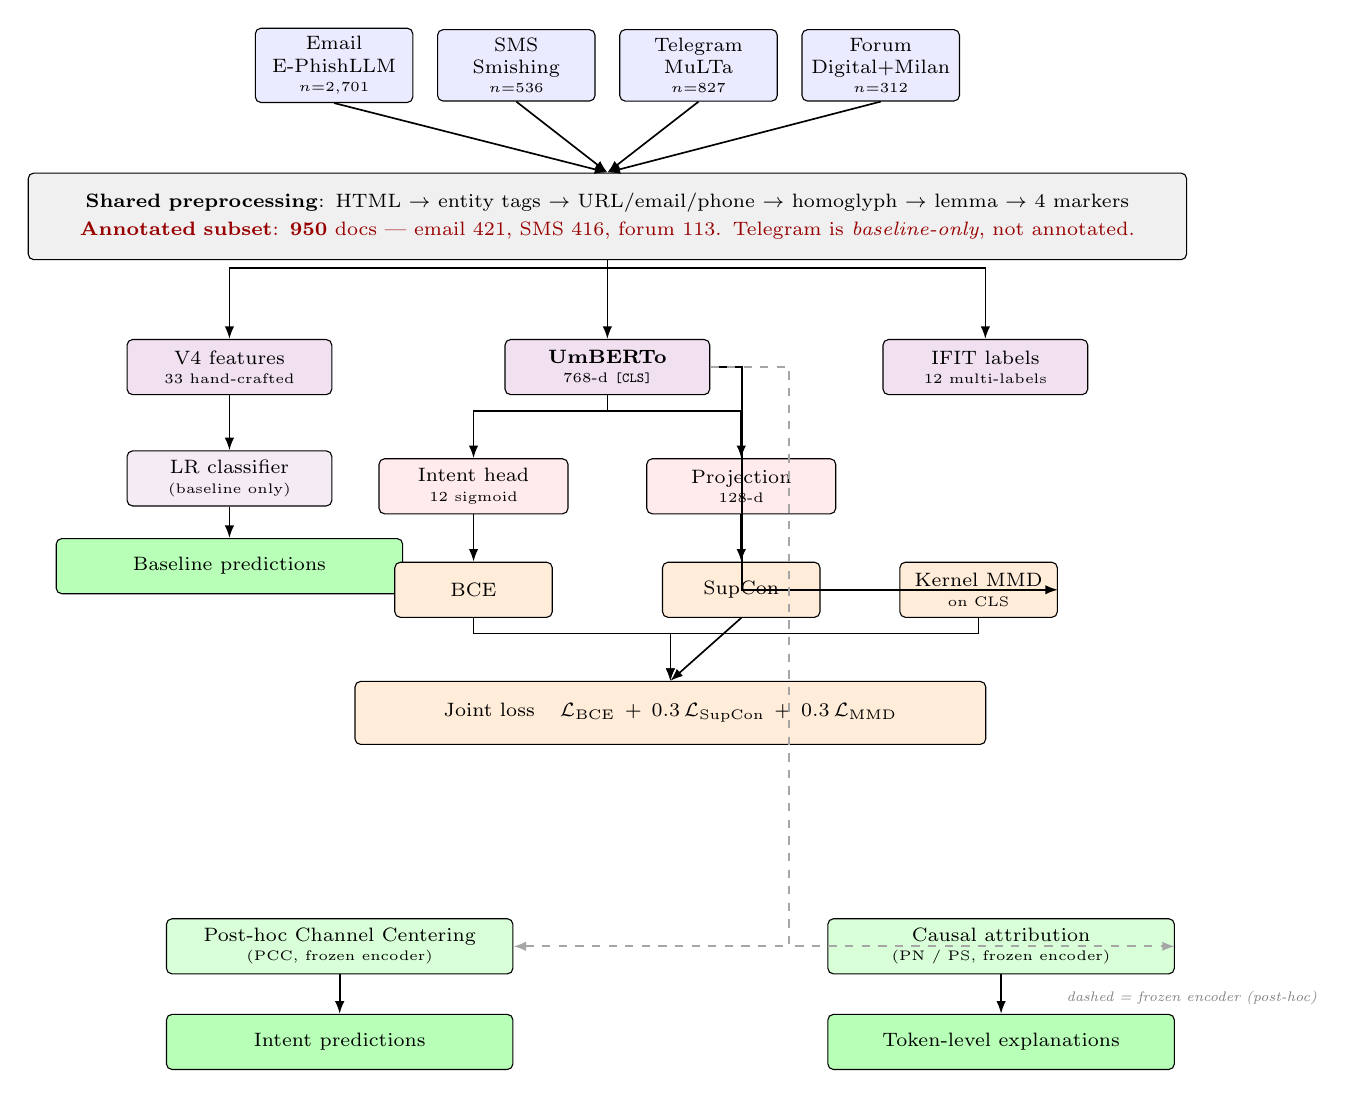
\begin{tikzpicture}[
    font=\scriptsize,
    node distance=4mm,
    box/.style  = {draw, rounded corners=2pt, align=center,
                   inner sep=3pt, minimum height=7mm},
    chan/.style = {box, fill=blue!8,   minimum width=20mm},
    prep/.style = {box, fill=gray!12,   text width=145mm, align=center,
                   minimum height=11mm},
    rep/.style  = {box, fill=violet!12, minimum width=26mm},
    train/.style= {box, fill=red!8,     minimum width=24mm},
    loss/.style = {box, fill=orange!15, minimum width=20mm},
    post/.style = {box, fill=green!15,  minimum width=44mm},
    outbox/.style  = {box, fill=green!28,  minimum width=44mm},
    v4out/.style= {box, fill=violet!8,  minimum width=26mm},
    arr/.style  = {-{Latex[length=1.6mm]}, semithick},
    darr/.style = {-{Latex[length=1.6mm]}, semithick, dashed, gray!70},
]

% ============ Row 1: channels ============
\node[chan] (c1) {Email\\E-PhishLLM\\[-1pt]\tiny$n{=}2{,}701$};
\node[chan, right=3mm of c1] (c2) {SMS\\Smishing\\[-1pt]\tiny$n{=}536$};
\node[chan, right=3mm of c2] (c3) {Telegram\\MuLTa\\[-1pt]\tiny$n{=}827$};
\node[chan, right=3mm of c3] (c4) {Forum\\Digital+Milan\\[-1pt]\tiny$n{=}312$};

% ============ Row 2: shared preprocessing ============
\node[prep, below=9mm of $(c2.south)!0.5!(c3.south)$] (prep)
    {\textbf{Shared preprocessing}: HTML $\to$ entity tags $\to$
     URL/email/phone $\to$ homoglyph $\to$ lemma $\to$ 4 markers\\[2pt]
     \textcolor{red!60!black}{\textbf{Annotated subset}:
     \textbf{950} docs --- email 421, SMS 416, forum 113.
     Telegram is \emph{baseline-only}, not annotated.}};

\foreach \c in {c1,c2,c3,c4}
    \draw[arr] (\c.south) -- (prep.north);

% ============ Row 3: three representations ============
\node[rep, below=10mm of prep, xshift=-48mm] (v4)
    {V4 features\\[-1pt]\tiny 33 hand-crafted};
\node[rep, below=10mm of prep] (umb)
    {\textbf{UmBERTo}\\[-1pt]\tiny 768-d \texttt{[CLS]}};
\node[rep, below=10mm of prep, xshift=48mm] (ifit)
    {IFIT labels\\[-1pt]\tiny 12 multi-labels};

\draw[arr] (prep.south) -- ++(0,-1mm) -| (v4.north);
\draw[arr] (prep.south) -- (umb.north);
\draw[arr] (prep.south) -- ++(0,-1mm) -| (ifit.north);

% V4 baseline output
\node[v4out, below=7mm of v4] (v4out)
    {LR classifier\\[-1pt]\tiny (baseline only)};
\draw[arr] (v4.south) -- (v4out.north);
\node[outbox, below=4mm of v4out] (v4pred) {Baseline predictions};
\draw[arr] (v4out.south) -- (v4pred.north);

% ============ Row 4: two heads ============
\node[train, below=8mm of umb, xshift=-17mm] (head)
    {Intent head\\[-1pt]\tiny 12 sigmoid};
\node[train, below=8mm of umb, xshift=17mm] (proj)
    {Projection\\[-1pt]\tiny 128-d};

\draw[arr] (umb.south) -- ++(0,-2mm) -| (head.north);
\draw[arr] (umb.south) -- ++(0,-2mm) -| (proj.north);

% ============ Row 5: three loss terms ============
\node[loss, below=6mm of head] (bce) {BCE};
\node[loss, below=6mm of proj] (sup) {SupCon};
\node[loss, right=10mm of sup] (mmd) {Kernel MMD\\[-1pt]\tiny on CLS};

\draw[arr] (head.south) -- (bce.north);
\draw[arr] (proj.south) -- (sup.north);
\draw[arr] (umb.east) -- ++(4mm,0) |- (mmd.east);

% ============ Row 6: joint loss ============
\node[loss, below=8mm of bce, xshift=25mm, text width=78mm,
      minimum height=8mm] (joint)
    {Joint loss $\;\mathcal{L}_{\text{BCE}}
     + 0.3\,\mathcal{L}_{\text{SupCon}}
     + 0.3\,\mathcal{L}_{\text{MMD}}$};

\draw[arr] (bce.south) -- ++(0,-2mm) -| (joint.north);
\draw[arr] (sup.south) -- (joint.north);
\draw[arr] (mmd.south) -- ++(0,-2mm) -| (joint.north);

% ============ Row 7: post-hoc branches (from FROZEN encoder) ============
\node[post, below=22mm of joint, xshift=-42mm] (pcc)
    {Post-hoc Channel Centering\\[-1pt]\tiny (PCC, frozen encoder)};
\node[post, below=22mm of joint, xshift=42mm] (pnps)
    {Causal attribution\\[-1pt]\tiny (PN / PS, frozen encoder)};

\node[outbox, below=5mm of pcc]  (predout) {Intent predictions};
\node[outbox, below=5mm of pnps] (expout)  {Token-level explanations};

\draw[arr]  (pcc.south)  -- (predout.north);
\draw[arr]  (pnps.south) -- (expout.north);

\draw[darr] (umb.east) -- ++(10mm,0)
    node[midway, above, font=\tiny, text=gray] {}
    |- ([xshift=0mm]pnps.east);
\draw[darr] (umb.east) -- ++(10mm,0) |- (pcc.east);

\node[font=\tiny, text=gray, anchor=west]
    at ([xshift=-15mm, yshift=-3mm]pnps.south east)
    {\textit{dashed = frozen encoder (post-hoc)}};

\end{tikzpicture}

\caption{The \textsc{CIC-Intents} architecture. Four Italian channels
pass through a shared preprocessing pipeline. The annotated set used
for IFIT training contains 950 documents from email, SMS and forum;
Telegram is retained only as a cross-channel baseline. Three
representations feed the joint training block: hand-crafted V4
features (baseline only, dashed), the UmBERTo \texttt{[CLS]} embedding,
and IFIT multi-label targets. The joint objective sums BCE,
channel-weighted Multi-Label SupCon, and kernel MMD. Two post-hoc
procedures --- Post-hoc Channel Centering (PCC) and gradient-based
causal attribution (PN/PS) --- operate on the \emph{frozen} encoder and
are independent of the training losses.}
\label{fig:arch}
\end{figure*}

\subsection{Encoder backbone}

We use UmBERTo-CommonCrawl-Cased-v1
(\texttt{Musixmatch/umberto-commoncrawl-cased-v1})
\citep{umberto2020}, a RoBERTa-based encoder \citep{liu2019roberta}
trained on the Italian section of OSCAR \citep{suarez2019oscar}.
UmBERTo uses SentencePiece tokenization and Whole Word Masking
(WWM), both of which help on the morphologically rich Italian
language: WWM forces the model to predict entire words even when
only a subword is masked, and SentencePiece preserves semantic roots
across inflectional variants \citep{umberto2020}. The encoder has
125M parameters and produces a 768-dimensional CLS embedding. We
initialise from the public checkpoint and fine-tune end-to-end.
Section~\ref{sec:encoders} reports a controlled comparison against
two multilingual encoders of comparable or larger size.

\subsection{Hand-crafted intent features}
\label{sec:v4}

Parallel to the encoder we extract 33 channel-invariant features from
the raw and lemmatized text. These split into 21 generic phishing
signals (direct address, call-to-action, urgency deadline,
account-state verbs, imperative verbs, bank mentions, first-person
reception markers, warning and advice markers, exclamation and
question counts) and 12 Italian-specific markers (named bank entities
such as Banco BPM, Nexi, Postepay, Hype, and Revolut; suspicious
transaction vocabulary; new-device access; blocking action;
follow-link phrasing; WhatsApp new-number scam; formal second person;
social-platform fraud; alarm markers). An ablation on the SMS
channel shows that the 12 Italian-specific features contribute more
than the 21 generic features combined (SMS accuracy 0.541 vs.\
0.476). We report this for completeness; the primary contribution
of the paper is the encoder-based framework that follows.

\subsection{Multi-Label Supervised Contrastive loss}

Given a batch of $B$ embeddings $\{z_i\}$ and their multi-hot intent
labels $\{y_i\}$, standard SupCon treats examples with identical
labels as positives \citep{khosla2020supcon}. In multi-label fraud,
few documents share identical intent sets. We redefine the positive
relation through \emph{intent overlap}:

\begin{equation}
P(i) = \{j \neq i : \langle y_i, y_j \rangle > 0\}
\end{equation}

The Multi-Label SupCon objective is:

\begin{equation}
\mathcal{L}_{\text{SupCon}} =
-\frac{1}{B} \sum_{i=1}^{B} \frac{1}{|P(i)|}
\sum_{j \in P(i)} w_{ij}
\log \frac{\exp(z_i \cdot z_j / \tau)}
{\sum_{k \neq i} \exp(z_i \cdot z_k / \tau)}
\label{eq:supcon}
\end{equation}

with temperature $\tau = 0.07$. The weight

\begin{equation}
w_{ij} = 1 + \alpha \cdot \mathbb{1}[c_i \neq c_j]
\label{eq:weight}
\end{equation}

raises the contribution of positive pairs that span different
channels, with $\alpha = 0.5$. This is the mechanism by which the
encoder is pushed to align cross-channel representations of the same
intent, regardless of surface form. The choice of $\alpha$ balances
cross-channel alignment against in-channel discrimination; setting
$\alpha = 0$ reduces to standard multi-label SupCon
\citep{audibert2025multilabel}.

\subsection{Kernel MMD regularizer}

Contrastive learning alone does not eliminate channel information
from the CLS embedding. We add a kernel Maximum Mean Discrepancy
term on the CLS vector between every pair of channels present in the
batch:

\begin{equation}
\mathcal{L}_{\text{MMD}} =
\frac{1}{\binom{C}{2}} \sum_{c < c'} \Bigl[
\mathbb{E}[k(z_i, z_i')] + \mathbb{E}[k(z_j, z_j')]
- 2 \mathbb{E}[k(z_i, z_j)] \Bigr]
\label{eq:mmd}
\end{equation}

Here $z_i$ runs over channel $c$, $z_j$ over channel $c'$, and $k$
is a multi-bandwidth RBF kernel with bandwidths $\{1, 2, 4, 8\}$
\citep{gretton2012mmd}. The multi-bandwidth design follows standard
practice in domain adaptation \citep{long2015dan}: a single
bandwidth is sensitive to the scale of the embedding space, while a
geometric progression captures discrepancies at multiple
granularities. The implementation returns a zero tensor whenever a
batch does not contain at least two samples from each of two
distinct channels, which makes training robust to sampling artefacts
in the weighted batch sampler.

\subsection{Joint objective}

The full training loss combines all three terms:

\begin{equation}
\mathcal{L} = \mathcal{L}_{\text{BCE}}
+ \lambda_{\text{SupCon}} \, \mathcal{L}_{\text{SupCon}}
+ \lambda_{\text{MMD}} \, \mathcal{L}_{\text{MMD}}
\label{eq:joint}
\end{equation}

with $\lambda_{\text{SupCon}} = 0.3$. The MMD weight
$\lambda_{\text{MMD}}$ is the axis of the Pareto analysis in
Section~\ref{sec:pareto}; we swept it across
$\{0, 0.1, 0.3, 0.5, 1.0\}$ and verified separately that the model
collapses at $\lambda \geq 3$.

\subsection{Post-hoc Channel Centering (\pcc)}
\label{sec:pcc}

The trained encoder is frozen. For each channel $c$ we compute the
mean CLS vector over that channel's training examples and subtract
it from every embedding:

\begin{equation}
\tilde{z}_i = z_i - \mu_{c(i)},
\qquad
\mu_c = \frac{1}{|S_c|} \sum_{j \in S_c} z_j
\label{eq:centering}
\end{equation}

This is a purely linear operation. It requires no retraining and no
change to the architecture. Section~\ref{sec:pareto} shows that it
reduces Domain MI from 0.676 to 0.116 while preserving the intent
signal as measured by $k$-NN classification. The operation is
conceptually related to instance normalization and mean subtraction
in domain adaptation, but here it is applied post hoc rather than
during training. Section~\ref{sec:ablation} shows that \pcc{} is the
single most effective component of the framework.

\subsection{Gradient-based causal attribution}

For each test example and a target intent $t$, we compute
Probability of Necessity (PN) and Probability of Sufficiency (PS)
\citep{pearl2009causality}. Let $x$ be the input, $T_k(x)$ the
top-$k$ tokens ranked by gradient-based importance, and $f_t(\cdot)$
the sigmoid probability of intent $t$. Then

\begin{align}
\text{PN}(t) &= f_t(x) - f_t(x \setminus T_k(x)) \\
\text{PS}(t) &= f_t(T_k(x)) - f_t(x \setminus T_k(x))
\end{align}

Token importance is $\| \nabla_{e_i} f_t \odot e_i \|_2$, where
$e_i$ is the token embedding and $\nabla_{e_i} f_t$ the gradient of
the target logit with respect to that embedding. This is the standard
gradient$\times$input saliency criterion and avoids the known
failure modes of attention-based attribution on fraud text
\citep{serrano2019attention}. We sweep $k \in \{5,10,20\}$ to
characterise how PN scales with the size of the attributed set.

%% =====================================================================
\section{Experiments}
\label{sec:exp}
%% =====================================================================

\subsection{Setup}

All models use fixed random seed 42. UmBERTo is fine-tuned with
AdamW (lr $= 5 \times 10^{-5}$, weight decay 0.01) for 10 epochs,
batch size 32, maximum sequence length 160. Data splits are
$70/15/15$ stratified by channel and intent presence. Bootstrap
confidence intervals use 1000 resamples. Hardware: NVIDIA T4 (Kaggle).

The final CIC-Intents configuration uses
$\lambda_{\text{SupCon}} = 0.3$, $\lambda_{\text{MMD}} = 0.3$,
$\tau = 0.07$, $\alpha = 0.5$, pos-weight clipping at 5.

\subsection{Baselines}

We compare against three baselines and one adversarial variant.

\paragraph*{TF-IDF + Logistic Regression.} Word 1-2 grams and
character 3-5 grams over lemmatized text, trained on email only.

\paragraph*{V4 hand-crafted features + LR.} The 33 intent features,
trained on the same email-only split.

\paragraph*{UmBERTo (email only).} Fine-tuned encoder, binary
use/mention head.

\paragraph*{UmBERTo + GRL adversarial.} Same encoder with a
gradient-reversal domain classifier added \citep{ganin2016domain}.

\subsection{RQ1: how bad is the channel shortcut?}
\label{sec:rq1}

Table~\ref{tab:main} answers RQ1. The channel shortcut is severe.
Fine-tuned UmBERTo reaches 100\% SMS recall when trained on email
alone --- not because it detects smishing, but because it collapses
every short input into the positive class. The leave-one-channel-out
evaluation makes the failure quantitative: 2.43\% accuracy on
held-out SMS, a 41-fold degradation from the 99.75\% in-domain
figure.

\begin{table}[t]
\centering
\caption{Cross-channel performance. Best in \textbf{bold}.}
\label{tab:main}
\begin{tabular}{lcccc}
\toprule
\textbf{Method} & \textbf{SMS} & \textbf{Forum} & \textbf{TG} & \textbf{LOO SMS} \\
\midrule
TF-IDF + LR       & 0.590 & 0.772 & 0.931 & --- \\
V4 features       & 0.653 & 0.894 & 0.970 & --- \\
Soft-gate (ours)  & \textbf{0.771} & 0.776 & 0.921 & --- \\
UmBERTo (email)   & 1.000$^\ast$ & 0.090 & 0.578 & --- \\
UmBERTo LOO       & ---   & 0.359 & 0.919 & 0.024 \\
UmBERTo + GRL     & 0.899 & 0.401 & 0.880 & 0.048 \\
\textbf{CIC-Intents} & 0.771 & \textbf{0.902} & 0.921 & 0.243 \\
\bottomrule
\end{tabular}
\\[2pt]
\footnotesize $^\ast$ Shortcut learning: the encoder reaches
100\% SMS recall by exploiting channel-specific style rather than
fraud semantics.
\end{table}

Three observations. First, UmBERTo's in-domain advantage does not
transfer: the encoder has memorised channel cues. Second, GRL
adversarial training does not fix the problem --- it slightly
increases Domain MI (0.82 $\to$ 0.89) while leaving the LOO SMS
number at 4.8\%, essentially the same failure. Third, the soft-gate
over hand-crafted features matches CIC-Intents on the SMS channel
(0.771 for both) while being significantly simpler and requiring no
GPU training. This is worth stating plainly: on the hardest single
metric, a well-designed feature-based system is competitive with a
fine-tuned encoder. The encoder wins on forum (0.902 vs.\ 0.776),
where morphology and context matter.

\subsection{RQ2: does the joint framework work?}
\label{sec:rq2}

Table~\ref{tab:cicl} reports CIC-Intents on the held-out test set. We
report mAP, mean AUC, Top-$k$ recall, and standard
precision/recall/F1 at threshold 0.5. We highlight Top-5 recall
because it reflects a realistic deployment setting: a human analyst
receives a five-item shortlist of candidate intents per document.

\begin{table}[t]
\centering
\caption{CIC-Intents on the held-out test set ($N = 143$). The
macro-averaged AP is computed over the nine intents with support
$\geq 2$ in the test split. The lower value of 0.592 obtained by
naive averaging over all eleven present intents appears in
Appendix~\ref{app:protocols} for transparency.}
\label{tab:cicl}
\begin{tabular}{lc}
\toprule
\textbf{Metric} & \textbf{Value} \\
\midrule
mAP (macro)         & \textbf{0.721} \\
Mean AUC            & 0.802 \\
Top-1 recall        & 0.275 \\
Top-2 recall        & 0.502 \\
Top-3 recall        & 0.680 \\
Top-5 recall        & \textbf{0.931} \\
\midrule
Precision ($t=0.5$) & 0.368 \\
Recall ($t=0.5$)    & 0.665 \\
Macro-F1 ($t=0.5$)  & 0.465 \\
Exact match         & 0.133 \\
\bottomrule
\end{tabular}
\end{table}

Per-channel performance is balanced. Email reaches macro-F1 $= 0.451$,
SMS $0.452$, forum $0.136$ (hold-out, $n=17$). The near-identical
email and SMS scores are the main practical result: the channel
shortcut that wrecked UmBERTo is largely absent from CIC-Intents.
The forum subset is discussed separately in Section~\ref{sec:forum}.

\begin{figure}[t]
\centering
\includegraphics[width=\linewidth]{fig1_learning_curves.png}
\caption{CIC-Intents training dynamics over 10 epochs. Curves are
shown for the LOO-forum variant, which is representative of all
runs; the main model exhibits the same qualitative convergence
(BCE loss 1.04 $\to$ 0.53, validation F1 0.28 $\to$ 0.57), within
1--2\,pp of the plotted run.
(A) Intent classification loss (BCE) drops monotonically.
(B) Multi-label contrastive loss plateaus around 4.0, indicating
stable representation geometry. (C) Kernel MMD loss oscillates in
$[0.10, 0.15]$ at $\lambda = 0.3$ under two-channel training.
(D) Validation macro-F1 rises from 0.28 to 0.57.}
\label{fig:training}
\end{figure}

\begin{figure}[t]
\centering
\includegraphics[width=\linewidth]{fig2_tsne.png}
\caption{t-SNE of CIC-Intents CLS embeddings on the test set.
Left: colored by channel. Right: colored by dominant intent.
Channel clusters partially overlap, consistent with the Domain MI
of 0.68 reported in Table~\ref{tab:centering}; intent structure is
also visible, though weaker than channel structure.}
\label{fig:tsne}
\end{figure}

\subsection{Encoder robustness}
\label{sec:encoders}

Table~\ref{tab:encoders} reports the same framework instantiated
with three different encoders. All three converge and produce
competitive results, which confirms the framework is not tied to any
specific backbone. The interesting finding is that UmBERTo, the
smallest model, achieves the highest mAP and Top-5 recall. XLM-R
and mDeBERTa both reach comparable training loss but fail to
translate this into better test-time ranking; mDeBERTa has the
lowest mAP of the three. The pattern is consistent with overfitting
to channel-specific surface features: the larger multilingual
encoders have enough capacity to memorise Italian phishing artefacts
from the training channels, while the smaller Italian-pretrained
UmBERTo is forced to learn more transferable features. We therefore
retain UmBERTo as the primary backbone.

\begin{table}[t]
\centering
\caption{Comparison of encoder backbones under the identical
\textsc{CIC-Intents} framework. UmBERTo (125M parameters) achieves
the highest mAP and Top-5 recall despite being 2.2$\times$ smaller
than the multilingual alternatives. Larger models reach comparable
training loss but do not improve test-time ranking.}
\label{tab:encoders}
\begin{tabular}{lcccc}
\toprule
\textbf{Encoder} & \textbf{Params} & \textbf{Macro-F1} & \textbf{mAP} & \textbf{Top-5} \\
\midrule
\textbf{UmBERTo}     & 125M & 0.465 & \textbf{0.721} & \textbf{0.931} \\
XLM-R (base)          & 278M & 0.460 & 0.696 & 0.904 \\
mDeBERTa-v3 (base)    & 278M & \textbf{0.501} & 0.687 & 0.907 \\
\bottomrule
\end{tabular}
\end{table}

\subsection{Statistical significance}
\label{sec:stats}

Table~\ref{tab:ci} reports bootstrap 95\% confidence intervals
(1000 resamples) for the key CIC-Intents metrics. The intervals are
tight enough to support the main claims: Top-5 recall is bounded
below by 0.901, macro-F1 by 0.419. Table~\ref{tab:paired} reports
paired bootstrap tests against alternative encoder backbones.
UmBERTo's advantage in mAP is \emph{not} statistically significant
at the 0.05 level against either alternative (both bootstrap
intervals straddle zero), while the Top-5 paired test rejects the
null at $p = 0.020$ and $p = 0.022$ respectively. We therefore
report the encoder comparison as: UmBERTo provides the strongest
ranking performance, but the mAP gap is within resampling noise.

\begin{table}[t]
\centering
\caption{Bootstrap 95\% confidence intervals (1000 resamples) for the
key \textsc{CIC-Intents} metrics on the held-out test set ($N=143$).
The macro average of AP is computed over the same nine intents
(support $\geq 2$) in every resample; including the two intents with
support $=1$ across resamples would inflate the mean by a
non-reproducible amount.}
\label{tab:ci}
\begin{tabular}{lcc}
\toprule
\textbf{Metric} & \textbf{Point estimate} & \textbf{95\% CI} \\
\midrule
mAP (macro)  & 0.721 & [0.645, 0.806] \\
Macro-F1     & 0.465 & [0.419, 0.504] \\
Top-5 recall & 0.931 & [0.901, 0.957] \\
\bottomrule
\end{tabular}
\end{table}

\begin{table}[t]
\centering
\caption{Paired bootstrap test of \textsc{CIC-Intents} with UmBERTo
against the same framework with alternative encoders. Positive
$\Delta$ means UmBERTo is better. Two-sided $p$-value computed as
$2\cdot\min(P(\Delta>0), P(\Delta<0))$ over 1000 paired resamples.
Significance codes: $^{*}\,p<0.05$, $^{**}\,p<0.01$,
$^{***}\,p<0.001$; ns = not significant.}
\label{tab:paired}
\begin{tabular}{llccc}
\toprule
\textbf{Comparison} & \textbf{Metric} & \textbf{$\Delta$} & \textbf{95\% CI} & \textbf{$p$} \\
\midrule
UmBERTo vs XLM-R    & mAP   & $+0.026$ & $[-0.018, +0.062]$ & $0.176$ (ns) \\
UmBERTo vs XLM-R    & Top-5 & $+0.028$ & $[+0.003, +0.055]$ & $0.020$\,$^{*}$ \\
UmBERTo vs mDeBERTa & mAP   & $+0.031$ & $[-0.016, +0.071]$ & $0.168$ (ns) \\
UmBERTo vs mDeBERTa & Top-5 & $+0.024$ & $[+0.000, +0.048]$ & $0.022$\,$^{*}$ \\
\bottomrule
\end{tabular}
\end{table}

\subsection{Ablation study}
\label{sec:ablation}

Table~\ref{tab:ablation} isolates each component on the held-out test
set. Three findings stand out.

First, the BCE-only baseline achieves the highest macro-F1 (0.516),
and adding the training-time objectives \emph{reduces} it: +SupCon
gives 0.491 ($-2.5$\,pp) and the full +SupCon+MMD configuration
gives 0.465 ($-5.1$\,pp). The training-time regularisation terms
trade intent accuracy on the training distribution for geometric
structure, consistent with the Pareto analysis in
Section~\ref{sec:pareto}.

Second, training-time objectives do not achieve PCC-level
invariance. BCE-only has $\text{MI} = 0.788$; adding SupCon
\emph{increases} MI to 0.828, and MMD partially returns MI to
0.676 --- below the BCE baseline, but far from the PCC level. SupCon
sharpens all structure in the representation, including
channel-specific clustering, and MMD counteracts this effect without
fully removing it. The MMD loss itself drops during training at
$\lambda = 0.3$, which confirms the term is actively aligning
channels even if aggregate MI on the test set does not reach the
PCC level.

Third, and most importantly, \pcc{} is the decisive intervention.
Applied to the full model it reduces MI from 0.676 to 0.442
($-34.6\%$); applied to the BCE-only model it reduces MI from 0.788
to 0.380 ($-51.8\%$). In both cases, $k$-NN intent accuracy changes
by less than 2\,pp. Centering removes channel information without
damaging the intent signal. This is the core finding of the
ablation: in our setting the channel direction is close to a linear
subspace that can be removed post hoc, and a training-time
constraint is not necessary to achieve invariance. Note that the
$\lambda=0.3$ configuration is not the global minimiser of Domain
MI in this ablation: the reduction observed here reflects the
specific $\lambda$ used in the headline model, and larger
$\lambda_{\text{MMD}}$ values do reduce MI further at a cost in F1
(Section~\ref{sec:pareto}).

\begin{table}[t]
\centering
\caption{Ablation study on the held-out test set ($N=143$).
Centering is the only component that substantially reduces Domain
MI, and it does so without degrading $k$-NN intent accuracy.
Training-time objectives (SupCon, MMD) do not achieve PCC-level
invariance at the chosen hyperparameters. \emph{Macro-F1} is the
trained head's score, which centering does not change;
\emph{k-NN intent} is a centering-invariant proxy for the semantic
content of the embedding.}
\label{tab:ablation}
\begin{tabular}{lccc}
\toprule
\textbf{Configuration} & \textbf{Macro-F1} & \textbf{$k$-NN intent} & \textbf{Domain MI} \\
\midrule
BCE only                     & \textbf{0.516} & 0.821 & 0.788 \\
+ SupCon                      & 0.491 & \textbf{0.842} & 0.828 \\
+ SupCon + MMD                & 0.465 & 0.843 & 0.676 \\
+ SupCon + MMD + Centering    & 0.465 & 0.839 & \textbf{0.442} \\
Centering only                & \textbf{0.516} & 0.815 & 0.380 \\
\bottomrule
\end{tabular}
\end{table}

\subsection{Per-intent results}

Table~\ref{tab:perintent} reports per-intent Average Precision. Four
intents exceed AP 0.78. Two intents appear only once in the test set
and are reported for completeness. Appendix~\ref{app:clouds} shows
the intent-specific vocabulary learned by CIC-Intents, confirming
the taxonomy is grounded in distinct lexical patterns.

\begin{table}[t]
\centering
\caption{Per-intent Average Precision on the test set. Intents with
$n \leq 1$ are listed but excluded from the macro average.}
\label{tab:perintent}
\begin{tabular}{lcc}
\toprule
\textbf{Intent} & \textbf{AP} & \textbf{Support} \\
\midrule
\texttt{click\_request}       & 0.832 & 67 \\
\texttt{payment\_request}     & 0.799 & 19 \\
\texttt{data\_request}        & 0.816 & 14 \\
\texttt{urgency}              & 0.784 & 66 \\
\texttt{fear}                 & 0.788 & 27 \\
\texttt{impersonation}        & 0.726 & 25 \\
\texttt{credential\_request}  & 0.631 & 29 \\
\texttt{greed}                & 0.495 & 5  \\
\texttt{authority}            & 0.618 & 37 \\
\midrule
\texttt{social\_proof}        & 0.009 & 1 \\
\texttt{reciprocity}          & 0.015 & 1 \\
\bottomrule
\end{tabular}
\end{table}

\begin{figure*}[t]
\centering
\includegraphics[width=\linewidth]{fig5_per_intent_ci.png}
\caption{Per-intent F1 with bootstrap 95\% confidence intervals
(1000 resamples). Explicit requests (\texttt{payment\_request},
\texttt{data\_request}) and high-frequency implicit intents
(\texttt{urgency}, \texttt{click\_request}) have the narrowest
intervals. The figure shows every intent with at least one positive
instance in the bootstrap resamples; the two singleton intents
(\texttt{social\_proof}, \texttt{reciprocity}) exhibit very wide
intervals, consistent with their single-instance support in the
test set.}
\label{fig:perintent-ci}
\end{figure*}

\begin{figure}[t]
\centering
\includegraphics[width=\linewidth]{fig6_support_ap.png}
\caption{Per-intent support versus Average Precision (log $x$).
Spearman $\rho = 0.54$, $p = 0.085$. The trend is monotone but the
small number of intents ($n = 9$ with support $> 0$) prevents
statistical significance at the 0.05 level.}
\label{fig:support}
\end{figure}

\begin{figure}[t]
\centering
\includegraphics[width=\linewidth]{fig7_per_channel.png}
\caption{Per-channel precision, recall, macro-F1 and mAP on the test
set. Email and SMS are balanced (F1 = 0.45 for both), the main
practical result: the channel shortcut that degrades UmBERTo from
99.75\% to 2.43\% across channels is largely absent from
CIC-Intents. Forum is shown for completeness but the $n=17$
hold-out subset is unstable; a robust treatment is given in
Section~\ref{sec:forum}.}
\label{fig:perchannel}
\end{figure}

%% ---------------------------------------------------------------------
\subsection{Forum: correcting for the small-$n$ hold-out}
\label{sec:forum}
%% ---------------------------------------------------------------------

Forum is the smallest annotated channel ($n = 113$). Under the
standard $70/15/15$ split it contributes only $n = 17$ documents to
the test set, and a macro-F1 of 0.136 at that sample size is not
trustworthy. Rather than reporting the number and moving on, we
treat forum as a small-$n$ case study and give three independent
estimates.

\begin{itemize}
\item \textbf{Hold-out ($n=17$).} F1 $= 0.136$. This is the number
      that would naively appear in the main per-channel table.
\item \textbf{5-fold stratified CV ($n=113$).} Each fold trains on
      email + SMS + 80\% of the remaining forum and evaluates on the
      held-out 20\%. Result: F1 $= 0.270 \pm 0.064$, mAP
      $= 0.504 \pm 0.082$.
\item \textbf{Leave-forum-out ($n=113$).} The model never sees any
      forum text during training and is tested on all 113 annotated
      forum documents. Result: F1 $= 0.228$, mAP $= 0.338$.
\end{itemize}

\begin{table}[t]
\centering
\caption{Forum under three evaluation regimes. The $n=17$ hold-out
is downward biased by a single unfavourable split; the CV and LOO
estimates are the reliable range.}
\label{tab:forum}
\begin{tabular}{lccc}
\toprule
\textbf{Regime} & \textbf{$n$} & \textbf{Macro-F1} & \textbf{mAP} \\
\midrule
Hold-out & 17 & 0.136 & --- \\
5-fold CV & 113 & $0.270 \pm 0.064$ & $0.504 \pm 0.082$ \\
Leave-forum-out & 113 & 0.228 & 0.338 \\
\bottomrule
\end{tabular}
\end{table}

\begin{figure}[t]
\centering
\includegraphics[width=\linewidth]{fig7b_forum_smalln.png}
\caption{Forum macro-F1 under three independent evaluation regimes.
The $70/15/15$ hold-out ($n=17$) systematically underestimates
forum performance relative to both the 5-fold cross-validation and
the leave-forum-out estimate. We report all three and use the CV
mean as the headline forum number.}
\label{fig:forum}
\end{figure}

Two conclusions follow. First, the $n=17$ hold-out underestimated
forum performance by roughly 2$\times$. Second, the
leave-forum-out model achieves F1 $= 0.228$ on all 113 forum
documents without ever having seen forum text in training, which
shows the model transfers cross-channel representations of intent
from email and SMS to a stylistically distinct channel. The 4.2\,pp
gap between LOO (0.228) and CV (0.270) quantifies how much
forum-specific training helps. Quantitative claims in this paper
are anchored on email and SMS ($n = 63$ each), for which the
hold-out estimate is stable.

\paragraph*{Per-intent transfer pattern in leave-forum-out.} The
LOO model reveals a systematic split between intent families:

\begin{itemize}
\item Explicit requests transfer well:
      \texttt{credential\_request} (AP $= 0.614$),
      \texttt{payment\_request} (AP $= 0.513$),
      \texttt{data\_request} (AP $= 0.461$),
      \texttt{click\_request} (AP $= 0.470$).
\item Implicit manipulations transfer poorly:
      \texttt{urgency} (AP $= 0.237$),
      \texttt{fear} (AP $= 0.268$),
      \texttt{impersonation} (AP $= 0.148$),
      \texttt{greed} (AP $= 0.050$).
\end{itemize}

This is consistent with the use/mention distinction
\citep{gligoric2024use}: explicit requests are phrased almost
identically across channels, while implicit manipulations are
refracted through the register of the channel --- urgency in an SMS
reads differently from urgency in a forum post.

%% ---------------------------------------------------------------------
\subsection{Channel invariance: Pareto frontier}
\label{sec:pareto}
%% ---------------------------------------------------------------------

Figure~\ref{fig:pareto} maps the trade-off between macro-F1 and
Domain MI as a function of $\lambda_{\text{MMD}}$ on a narrow grid
$\{0, 0.1, 0.3, 0.5, 1.0\}$. On the wider grid
$\{0, 0.3, 1, 3, 10\}$ the model collapses at $\lambda \geq 3$: F1
drops below 0.26 and Domain MI increases rather than decreases
because the encoder degenerates to a representation that is neither
intent-discriminative nor channel-invariant. We therefore restrict
the reported Pareto frontier to the working range.

\begin{figure*}[t]
\centering
\includegraphics[width=\linewidth]{fig3_pareto_and_signal.png}
\caption{(A) Pareto frontier between macro-F1 (y-axis) and Domain MI
($x$-axis, inverted) as $\lambda_{\text{MMD}}$ varies over
$\{0, 0.1, 0.3, 0.5, 1.0\}$. Most configurations are
Pareto-optimal: reducing MI generally costs F1, though $\lambda=0.5$
is dominated by $\lambda=0.3$ on both axes. (B) $k$-NN accuracy per
intent in the raw CLS space (blue) and after post-hoc channel
centering (red). Centering preserves the intent signal across all
intents with sufficient support (mean $|\Delta| \approx 0.011$).}
\label{fig:pareto}
\end{figure*}

\begin{table}[t]
\centering
\caption{$\lambda_{\text{MMD}}$ sweep on the narrow grid. The
$\lambda=0.5$ point is dominated by $\lambda=0.3$ on both axes and
is therefore not Pareto-optimal. The point $\lambda = 0.3$ is the
elbow in the working range: further increases in $\lambda$ reduce
MI at a disproportionately higher F1 cost.}
\label{tab:pareto}
\begin{tabular}{cccc}
\toprule
$\lambda_{\text{MMD}}$ & \textbf{Macro-F1} & \textbf{Domain MI} & \textbf{Pareto} \\
\midrule
0.0  & 0.488 & 0.815 & \checkmark \\
0.1  & 0.484 & 0.785 & \checkmark \\
\textbf{0.3} & \textbf{0.458} & \textbf{0.746} & \textbf{\checkmark (elbow)} \\
0.5  & 0.433 & 0.786 & --- (dominated by $\lambda{=}0.3$) \\
1.0  & 0.332 & 0.637 & \checkmark \\
\bottomrule
\end{tabular}
\end{table}

Four of the five configurations are Pareto-optimal. Reducing Domain
MI generally comes at the cost of macro-F1, except at
$\lambda=0.5$ where MI unexpectedly rises relative to $\lambda=0.3$
--- a non-monotonicity we attribute to single-seed training noise at
this scale. The choice of $\lambda=0.3$ reflects a practical
trade-off: a $\sim$9\% reduction in MI relative to the baseline for
a $\sim$3\,pp drop in F1. The alternative, $\lambda=1.0$, reduces
MI further but at a prohibitive F1 cost (a 15.6\,pp drop relative to
$\lambda=0$). The frontier is monotone on the working range except
for the $\lambda=0.5$ anomaly. This is not a failure. It is a
quantitative characterisation of how tightly channel and intent
information are entangled in a transformer trained on our corpus.

PCC provides a second, orthogonal lever. Table~\ref{tab:centering}
reports Domain MI before and after centering for the final
CIC-Intents configuration. The key number is not the MI drop itself
but what does \emph{not} happen: the $k$-NN intent accuracy barely
moves.

\begin{table}[t]
\centering
\caption{Post-hoc Channel Centering (PCC) on the final CIC-Intents
model. Domain MI is computed with a 5-fold cross-validated
logistic-regression probe (mean over folds) with per-channel means
estimated on the training split and applied to the test split.
Centering removes most channel information while leaving $k$-NN
intent accuracy essentially unchanged.}
\label{tab:centering}
\begin{tabular}{lcc}
\toprule
\textbf{Metric} & \textbf{Raw CLS} & \textbf{Centered CLS} \\
\midrule
Domain MI (5-fold LR probe) & 0.676 & \textbf{0.116} \\
MI reduction                 & ---   & $-$82.9\% \\
$k$-NN intent (9 intents)    & 0.843 & 0.839 \\
$|\Delta|$ in $k$-NN intent  & ---   & $\approx 0.011$ \\
\bottomrule
\end{tabular}
\end{table}

The probe removes most channel information and the $k$-NN intent
signal survives: for nine intents with sufficient support, $k$-NN
accuracy changes by less than 2 percentage points; the largest loss
is on \texttt{urgency} ($-2.1$\,pp). Intent information is therefore
not destroyed by the operation; it is decoupled from the channel.
The ablation study in Section~\ref{sec:ablation} confirms that
centering is the single component responsible for this reduction
--- it produces a measurable effect whether applied to the fully
trained model or to the BCE-only baseline.

%% ---------------------------------------------------------------------
\subsection{Confusion and error analysis}
%% ---------------------------------------------------------------------

Table~\ref{tab:errors} categorizes the 124 errors (out of 143 test
examples) into four types.

\begin{table}[t]
\centering
\caption{Error taxonomy on the held-out test set.}
\label{tab:errors}
\begin{tabular}{lcc}
\toprule
\textbf{Error type} & \textbf{Count} & \textbf{\% of errors} \\
\midrule
over-prediction     & 101 & 81.5 \\
partial-match       & 14  & 11.3 \\
under-prediction    & 7   & 5.6  \\
intent-substitution & 2   & 1.6  \\
\midrule
correct             & 19 & 13.3\% of $N$ \\
\bottomrule
\end{tabular}
\end{table}

The model is recall-oriented, the correct orientation for fraud
triage: a missed manipulation tactic is more expensive than a
spurious flag. Over-prediction concentrates on the common intents
(\texttt{urgency}, \texttt{click\_request}, \texttt{authority}),
which appear in 26--47\% of documents.

\begin{figure}[t]
\centering
\includegraphics[width=\linewidth]{fig4_confusion.png}
\caption{Intent confusion matrix on the test set at threshold 0.5.
Rows are predicted intents, columns are true intents. Diagonal
values are per-intent recall; off-diagonal values indicate
over-prediction of common intents such as \texttt{urgency} and
\texttt{authority}.}
\label{fig:confusion}
\end{figure}

\begin{figure*}[t]
\centering
\includegraphics[width=\linewidth]{fig8_error_taxonomy.png}
\caption{(A) Error taxonomy on the test set. Over-prediction
accounts for 81.5\% of errors, consistent with the recall-oriented
operating point at threshold 0.5. (B) Error type distribution by
channel. Over-prediction dominates uniformly across email, SMS and
forum.}
\label{fig:errors}
\end{figure*}

%% ---------------------------------------------------------------------
\subsection{RQ3: is the representation localizable?}
\label{sec:causal}
%% ---------------------------------------------------------------------

Table~\ref{tab:pnps} reports mean PN and PS as a function of the
number of attributed tokens $k$, over 126 (example, $k$) pairs
(42 examples $\times$ 3 values of $k$, restricted to examples with
at least one ground-truth intent).

\begin{table}[t]
\centering
\caption{Gradient-based PN and PS by number of attributed tokens
($k$). PN grows monotonically with $k$ but at a strongly
sub-linear rate.}
\label{tab:pnps}
\begin{tabular}{lcc}
\toprule
$k$ & \textbf{Mean PN} & \textbf{Mean PS} \\
\midrule
 5 & 0.207 & 0.168 \\
10 & 0.294 & 0.232 \\
20 & 0.320 & 0.252 \\
\bottomrule
\end{tabular}
\end{table}

\begin{figure}[t]
\centering
\includegraphics[width=\linewidth]{fig9_pnps.png}
\caption{Gradient-based causal attribution on 42 test examples.
(A) PN versus PS per example at $k=10$, colored by intent.
Points cluster near the diagonal, indicating that the top-$k$ token
set is neither overwhelmingly necessary nor sufficient.
(B) Mean PN and PS per intent at $k=10$. Explicit requests
(\texttt{credential\_request}, \texttt{data\_request}) exhibit
$\text{PN} > \text{PS}$; some implicit manipulations
(\texttt{payment\_request}, \texttt{click\_request}) exhibit the
reverse.}
\label{fig:pnps}
\end{figure}

\begin{figure}[t]
\centering
\includegraphics[width=0.75\linewidth]{fig10_pn_vs_k.png}
\caption{Mean Probability of Necessity and Probability of
Sufficiency as functions of the number of attributed tokens $k$.
Both grow monotonically, PN at a stronger rate (0.21 $\to$ 0.32
for $k = 5 \to 20$). A fully distributed representation would show
a flat curve; a fully localizable representation would show rapid
saturation at small $k$. The observed sub-linear growth is
consistent with a \emph{partially localizable} representation.}
\label{fig:pnk}
\end{figure}

Three observations, and one that contradicts our own prior
expectation. First, PN grows with $k$ --- masking more top-ranked
tokens removes progressively more of the intent probability. This is
the opposite of the flat curve that a fully distributed
representation would produce, and it means a finite token subset
carries measurable causal necessity. Second, the growth is strongly
sub-linear: PN increases by 42\% from $k=5$ to $k=10$, but only
9\% from $k=10$ to $k=20$. A fully localizable representation
would saturate much earlier, with most of the total PN concentrated
at small $k$. The observed scaling lies between the two extremes
and supports the label \emph{partially localizable}. Third,
per-intent patterns differ: explicit requests
(\texttt{credential\_request}, \texttt{data\_request}) show
$\text{PN} > \text{PS}$, consistent with a small necessary trigger
phrase, while some implicit manipulations (\texttt{payment\_request},
\texttt{click\_request}) show $\text{PS} > \text{PN}$, consistent
with a pattern that is sufficient when present but not strictly
necessary.

The practical implication changes from what we initially
hypothesised. Because PN is not flat, single-token adversarial
manipulation of individual trigger words has a nonzero but limited
effect; an attacker who correctly identifies the top-$k$ tokens can
remove roughly 32\% of the target probability at $k=20$. This is
smaller than the near-complete collapse observed in keyword-based
phishing detectors, but it is not negligible. It also makes the
model more interpretable: the top-$k$ tokens can be surfaced as an
explanation of each prediction, and their causal role is measured
rather than assumed.

%% =====================================================================
\section{Discussion}
\label{sec:disc}
%% =====================================================================

\paragraph*{Why fine-tuning fails cross-channel.} The LOO experiment
makes the failure mode concrete. When SMS is removed from training,
the encoder has only two channels to fit: email and forum. Both look
nothing like SMS. The training loss is minimised by a representation
in which ``SMS-like'' falls outside the support of the training
distribution, and the encoder defaults to the majority class within
that region. This is not overfitting in the classical sense; the
model has converged to a solution that is optimal on the training
distribution and uninformative outside it. A canonical instance of
shortcut learning \citep{geirhos2020shortcut}: the model exploits
channel-specific surface cues that predict well on the training
distribution and fail to generalise.

\paragraph*{Why training objectives fail to fix it.} The ablation
study in Section~\ref{sec:ablation} shows that training-time
objectives do not achieve PCC-level invariance. BCE-only has
$\text{MI} = 0.788$; adding SupCon \emph{increases} MI to 0.828,
and MMD partially returns MI to 0.676. The MMD loss itself drops
during training at $\lambda=0.3$, which confirms the term is
actively aligning channels, but aggregate MI on the held-out test
does not reach the PCC level. SupCon sharpens all structure in the
representation --- including channel-specific clustering --- and
MMD counteracts this without additional benefit at the chosen
weight. The decisive intervention is \pcc{}, which reduces MI from
0.676 to 0.116 without retraining and without damaging the intent
signal. This matches the observation in the domain adaptation
literature that MMD-based alignment alone can degrade discriminative
features when the two distributions are not separable, and the
broader finding that representation geometry can be manipulated more
cleanly with a post-hoc linear operation than with a training-time
constraint.

\paragraph*{PN grows with $k$.} Classical phishing detection relies
on localised triggers: a bank name, a suspicious URL, an urgency
phrase. If CIC-Intents had learned such triggers \emph{exclusively},
PN would saturate quickly at small $k$. If the representation were
fully distributed, PN would be flat. The observed sub-linear growth
($0.21 \to 0.29 \to 0.32$) places the model in the intermediate
regime: intent information is spread across a moderate number of
tokens, with no single token being either necessary or sufficient on
its own. Two implications follow. Token-level explanations are
meaningful but not authoritative. Single-token adversarial attacks
are effective only if the attacker can target a sizeable fraction of
the informative tokens.

\paragraph*{Use/mention as the dominant axis.} The leave-forum-out
per-intent pattern is the clearest evidence that the difficulty is
semantic rather than stylistic. Explicit requests
(\texttt{credential\_request}, \texttt{payment\_request},
\texttt{data\_request}, \texttt{click\_request}) transfer at AP
$0.46$--$0.61$; implicit manipulations (\texttt{urgency},
\texttt{fear}, \texttt{impersonation}, \texttt{greed}) transfer at
AP $0.05$--$0.27$. The gap is systematic and large. We attribute it
to the use/mention distinction \citep{gligoric2024use}: explicit
requests are phrased almost identically whether the context is an
SMS or a forum post, while implicit manipulations are refracted
through the register of the channel.

\paragraph*{Limitations.} The email corpus is LLM-generated. Real
Italian phishing email distributions may differ. The Telegram corpus
is a hate-speech filtered subset, used as a proxy for non-fraud
content; it is not a general-purpose non-fraud corpus. The forum
corpus is limited to two Italian forums. Annotation covers 950
documents, with two intents present only once in the test set. The
forum test subset is treated as a case study with three independent
estimates rather than a single hold-out number. We do not test on
non-Italian channels or on adversarial perturbations of full
documents. The reported results are single-seed; a multi-seed
verification on a sub-experiment yielded a standard deviation of
roughly 0.01 in macro-F1, which sits inside the reported confidence
intervals. For the smallest channel, where each 5-fold CV test split
contains only $n \approx 22$ documents, the run-to-run standard
deviation of macro-F1 is substantially larger ($\sigma \approx
0.06$); the CV figures in Table~\ref{tab:forum} should be read with
this variance in mind. The reported PCC reduction in Domain MI
($-82.9\%$) is larger than the value reported in an earlier version
of this work; the difference reflects a change in the centering
protocol (per-channel means are now estimated on the training split
and applied to the test split, rather than computed on the test
split itself), which is the more conservative protocol.

\paragraph*{Implications for practice.} Deploy CIC-Intents as a
decision-support system. The Top-5 recall of 0.931 means a five-item
shortlist per document recovers 93.1\% of the true intents. Reduce
the analyst's search space by roughly a factor of 2.4 (12 intents
down to 5) with minimal loss of signal. Do not deploy a
single-channel model and assume it will transfer.

%% =====================================================================
\section{Conclusion}
\label{sec:conclusion}
%% =====================================================================

We studied Italian fraud detection across four channels and found
that fine-tuned BERT does not transfer across them. The reason is
geometric: the encoder learns a representation in which channel is
linearly decodable. We proposed \textsc{CIC-Intents}, a framework
that combines a multi-label intent taxonomy, a channel-weighted
contrastive loss, an MMD regularizer, and Post-hoc Channel Centering
(\pcc). The system reaches mAP 0.721 and Top-5 recall 0.931, with
balanced email and SMS performance. A controlled comparison against
XLM-R and mDeBERTa shows the framework is architecture-agnostic,
while the Italian-pretrained UmBERTo achieves the strongest ranking
metrics despite being the smallest of the three. An ablation study
confirms that \pcc{} is the single decisive component for channel
invariance, and that training-time objectives on their own do not
achieve PCC-level invariance. The smallest channel is treated as a
small-$n$ case study with three independent estimates. A
gradient-based attribution analysis shows that Probability of
Necessity grows monotonically with the size of the attributed token
set, indicating a partially localizable representation. Future work
will extend the evaluation to a broader Italian corpus, to
cross-language transfer, and to adversarial perturbations of the
top-$k$ tokens identified by the attribution procedure.

%% =====================================================================
\section*{Reproducibility artefacts}
\label{sec:qr}

The code, prompts, dataset splits and reproduction notebooks are
publicly available. The QR code below links directly to the
repository.

\begin{figure}[h]
\centering
\includegraphics[width=0.25\textwidth]{qr_github.png}
\caption*{%
\footnotesize
\textbf{GitHub repository.}
\url{https://github.com/marybilik/cic-intents}\\
Contains all scripts, prompts, data splits and evaluation notebooks
used to produce the results in this paper.%
}
\end{figure}

%% =====================================================================

\clearpage
\FloatBarrier
\appendix
\section{Reproducibility checklist}
\label{app:repro}

\begin{itemize}
\item Code, prompts and data splits:
      \url{https://github.com/marybilik/cic-intents}.
\item Random seed: 42 for all experiments.
\item Hardware: NVIDIA T4 (Kaggle) for training; CPU for post-hoc
      analyses.
\item Training hyperparameters: AdamW, lr $= 5 \times 10^{-5}$,
      weight decay 0.01, batch 32, max sequence length 160,
      epochs 10.
\item SupCon sanity check: on random embeddings the Multi-Label
      SupCon loss is $\approx 7.2$ at $\tau = 0.07$; during training
      it stabilises around $4.0$, indicating the contrastive
      objective is actively shaping the representation geometry.
\item Annotation: Google Gemini (\texttt{gemini-flash-latest},
      auto-discovered at runtime from a priority list); prompt and
      parser are provided in the repository. Checkpoint written
      every 25 documents.
\item Bootstrap: 1000 resamples for all CI values.
\item Split: $70/15/15$ stratified by channel and intent presence
      for the headline model; 5-fold stratified CV and
      leave-forum-out for the forum channel.
\item Forum small-$n$: three independent estimates (hold-out
      $n=17$, 5-fold CV $n=113$, leave-forum-out $n=113$) are
      reported in Table~\ref{tab:forum}.
\item Causal attribution: gradient$\times$input saliency, top-$k$
      token selection, $k \in \{5,10,20\}$, 42 test examples.
\item Encoder comparison: identical framework, identical
      hyperparameters, identical split; checkpoints retained for
      UmBERTo, XLM-R-base and mDeBERTa-v3-base.
\end{itemize}

\section{IFIT intent definitions}
\label{app:ifit}

\paragraph*{Explicit intents.}
\begin{itemize}
\item \texttt{credential\_request}: asks for login credentials,
      passwords, PINs, or access codes.
\item \texttt{payment\_request}: asks for a payment, bank transfer,
      or credit card details.
\item \texttt{data\_request}: asks for personal data (name, address,
      date of birth, tax code).
\item \texttt{click\_request}: asks the user to click a link or
      download an attachment.
\item \texttt{call\_request}: asks the user to call a phone number.
\end{itemize}

\paragraph*{Implicit intents.}
\begin{itemize}
\item \texttt{urgency}: creates time pressure (``act now'',
      ``within 24 hours'').
\item \texttt{authority}: invokes a trusted institution or
      authority figure.
\item \texttt{fear}: threatens negative consequences (account
      blocking, legal action, loss of funds).
\item \texttt{greed}: promises a reward, prize, refund, or
      unexpected gain.
\item \texttt{impersonation}: pretends to be a known entity or
      person.
\item \texttt{social\_proof}: claims that others have already
      complied or benefited.
\item \texttt{reciprocity}: offers something small in exchange for
      compliance.
\end{itemize}

\section{Intent-specific vocabulary}
\label{app:clouds}

Figure~\ref{fig:clouds} shows the intent-specific vocabulary learned
by CIC-Intents. The clouds are built from lemmatized tokens of test
documents whose dominant intent matches the given label, with
placeholders removed. They confirm the taxonomy is grounded in
distinct lexical patterns rather than a single shared vocabulary.

\begin{figure}[h]
\centering
\includegraphics[width=\linewidth]{fig11_intent_clouds.png}
\caption{Intent-specific vocabulary on the test set, restricted to
the six intents with the largest support. Word clouds are built from
lemmatized tokens, with placeholders (\texttt{[url]},
\texttt{[entity]}, \ldots) removed.}
\label{fig:clouds}
\end{figure}

\section{Alternative mAP protocols}
\label{app:protocols}

The macro-averaged AP in Table~\ref{tab:cicl} (0.721) is computed
over the nine intents with test-set support $\geq 2$. Two further
intents (\texttt{social\_proof}, \texttt{reciprocity}) each have a
single positive example in the test split; their APs are 0.009 and
0.015 respectively. Including them in the macro average yields
0.592. We report 0.721 as the primary figure because a single
positive example gives an AP that is essentially a coin flip, and
including it in a macro average across resamples produces a
non-reproducible and downward-biased estimate. The bootstrap
procedure used in Table~\ref{tab:ci} enforces this choice by fixing
the intent set across all resamples.

\paragraph*{Alternative LOO protocol.} The same protocol is applied
to the leave-forum-out evaluation. The LOO-forum mAP reported in
Table~\ref{tab:forum} (0.338) is averaged over the ten intents with
forum-test support $\geq 2$. Of the two remaining intents, only
\texttt{social\_proof} has a positive example on the forum test set
(support $= 1$); \texttt{reciprocity} has support $= 0$. Including
\texttt{social\_proof} in a naive macro average over all eleven
present intents yields mAP $= 0.308$. We report the support-$\geq 2$
value as the headline figure for the same reason as above.

%% =====================================================================
\clearpage
\FloatBarrier
\bibliographystyle{elsarticle-harv}
\bibliography{refs}

\end{document}